\documentclass[11pt]{article}

%PDF MetaData
\usepackage[pdftex,
	pdfauthor={Matthew Clark},
	pdftitle={An Introduction into Computer Vision: The Histogram of Oriented Gradients for Pedestrian Detection},
	pdfsubject={Computer Vision},
	pdfkeywords={HOG;Linear Algebra;Object Recognition},
	pdfproducer={pdfTeX-1.40.18},
	pdfcreator={LaTeX with hyperref package}]{hyperref}


%Packages
\usepackage{amsmath}
\usepackage{amssymb}
\usepackage{graphicx}

\usepackage{wrapfig}
\usepackage{subfig}
\usepackage{tikz}
\usepackage{caption}

\usepackage{setspace}
\usepackage{enumitem}
\usepackage{siunitx} % Required for alignment
\usepackage{multirow} % Required for multirows
\usepackage[utf8]{inputenc}
\usepackage{lmodern}
\usepackage{multicol}
\usepackage{helvet}
\renewcommand{\familydefault}{\sfdefault}

\usepackage{perpage} %the perpage package
\MakePerPage{footnote} %the perpage package command

%cite author
\usepackage[numbers]{natbib}

%Subtitle
\usepackage{titling}
\newcommand{\subtitle}[1]{
	\postauthor{
	\end{tabular}
		\par\end{center}
		\begin{center}
		\textit{\small#1}
		\end{center}
		\vskip0.5em
	}
}

%Math Packages
\usepackage{pgfplots}

%Math Commands
\newcommand{\eqname}[1]{\tag*{#1}}% Tag equation with name

\newcommand\numberthis{\addtocounter{equation}{1}\tag{\theequation}}%one equ label in align

%norm command
\newcommand{\norm}[1]{\left\lVert#1\right\rVert}


\makeatletter
\renewcommand*\env@matrix[1][*\c@MaxMatrixCols c]{%
	\hskip -\arraycolsep
	\let\@ifnextchar\new@ifnextchar
	\array{#1}}
\makeatother

\renewcommand*{\arraystretch}{0.8}

\makeatletter
\g@addto@macro\normalsize{%
	\setlength\abovedisplayskip{4pt}
	\setlength\belowdisplayskip{4pt}
	\setlength\abovedisplayshortskip{0pt}
	\setlength\belowdisplayshortskip{0pt}
}
\makeatother

\usepackage{mathtools}
\usepackage{chngcntr}
\counterwithin{equation}{section}

%Changes the Abstract title
\usepackage{abstract}
%\renewcommand{\abstractname}{Prompt}% Change the title

%Table Formatting
\sisetup{
round-mode          = places, % Rounds numbers
round-precision     = 2, % to 2 places
}

\usepackage{geometry}
\geometry{
a4paper,
total={216mm,279mm},
left=25.4mm,
right=25.4mm,
top=25.4mm,
bottom=25.4mm
}

%table of contents and paragraphs
\setcounter{secnumdepth}{5}
\setcounter{tocdepth}{5}

\let\orisectionmark\sectionmark
\renewcommand\sectionmark[1]{\label{sec:#1}\orisectionmark{#1}}

\let\orisubsectionmark\subsectionmark
\renewcommand\subsectionmark[1]{\label{subsec:#1}\orisubsectionmark{#1}}

\let\orisubsubsectionmark\subsubsectionmark
\renewcommand\subsubsectionmark[1]{\label{subsubsec:#1}\orisubsubsectionmark{#1}}

\newcommand\simpleparagraph[1]{%
	\stepcounter{paragraph}\paragraph*{\theparagraph\quad{}#1}}

\makeatletter
\renewcommand\thesubsubsection{}
\renewcommand\theparagraph{}
\makeatother

%horizontal line spacing
\usepackage{setspace}

\renewcommand{\baselinestretch}{1.0}


%paragraph title indent
%setlength{\parindent}{0}
%\setlength{\parskip}{0}

\begin{document}
		
%TitlePage
\title{\textbf{An Introduction into Computer Vision: The Histogram of Oriented Gradients for Pedestrian Detection}}
\author{\textbf{Matthew Clark}}
\subtitle{Computer Science Department\\
	The Masters University\\
	Santa Clarita, CA., United States\\
	mhckqw@gmail.com}
\date{\small May 15, 2018}
\maketitle
\vspace{1mm}

\begin{abstract}
	In recent years, due to significant improvements of sensors, processors, and image processing techniques, major milestones have been made in the field of autonomous vehicles. As a result, the automotive industry and consumers have developed a deep interest in the substantial socioeconomic impact autonomous vehicles have. To realize full autonomous driving, the vehicle must have reliable object detection systems. Lidar, cameras, and other proximity sensors are used to make this possible. Much of the current research and development is being poured into improving various object recognition techniques. A proper background and understanding of Computer Vision is vital to ensure advancement in applications like autonomous vehicles. To provide an effective tool to begin to understand the state of the field in its current form, this paper is devoted to the survey and analysis of the Histogram of Oriented Gradients technique.
\end{abstract}
\pagenumbering{gobble}	
\newpage

\pagenumbering{gobble}
\pagenumbering{arabic}
\newpage
\pagenumbering{gobble}
\tableofcontents

\newpage
\pagenumbering{arabic}
%vertical line spacing
%\onehalfspacing
\doublespacing
===
\section{Introduction} %Why is exploring the ethics of this very specific field important?
\simpleparagraph{}
Computer vision is a vast and far reaching field within computer science, and yet receives little recognition. Reflecting upon the significant milestones that represent the advancements of intelligent computing, a computer beating a chess grandmaster seems more \textit{intelligent} than a computer learning to recognize a face in an image. In reality, barely recognizing a face in an image had its first successes in the early 90's. A computer chess system was able to find success in 1970 against a chess grandmaster and was capable of beating people since the late 1950's \cite{contributors_computer_2018}. In the 1970's, it was believed that the ``visual input" problem for the ambitious goal of mimicking human intelligence was an easy task compared to problems involving higher-level reasoning and planning \cite{szeliski_computer_2011}. Those early pioneers soon realized the immense complexity and difficulty of computer vision.
\simpleparagraph{}
The  fundamental purpose of computer vision is to teach computers how to see \cite{nat_36_2017}\cite{malik_three_2016}. Studying computer vision, a field of applied math, requires geometry, calculus, linear algebra, probability, and machine learning. Despite the very narrow entryway, it is both academically enriching and a specialty that is extremely high in demand. Within the field of computer vision, object recognition is a relevant and integral application for autonomous vehicles. Although other applications of object recognition can be applied to surveillance systems, facial recognition, or intelligent photo editing. Within an autonomous vehicle system, object recognition is best suited for various tasks such as recognizing road lanes, surrounding vehicles, hazards, road signs, pedestrians, etc. To understand object recognition, this paper is devoted to providing a comprehensive review of the Histograms of Oriented Gradients technique\footnote{From now on the Histograms of Oriented Gradients will be refereed to as HOG} for Pedestrian Detection \cite{dalal_histograms_2005}, describing the necessary and foundational concepts.
\section{Image Processing}
\simpleparagraph{}
Before it is possible to understand the HOG \cite{dalal_histograms_2005} technique, a review of image processing is necessary. \textbf{Preprocessing}\label{Preprocessing} is the use of image processing to convert the input, an image, into a more suitable form for later analysis \cite{szeliski_computer_2011}. Generally the goal of preprocessing is to remove unnecessary data, correct the image, or alter its representation. Many of these tasks are computed using point operators, histograms, filters, gradients, or image pyramids. As a matter of fact, all of these tasks are necessary when using HOG.
\begin{figure}[h]
	\centering
	\subfloat[The Input Image]{%
		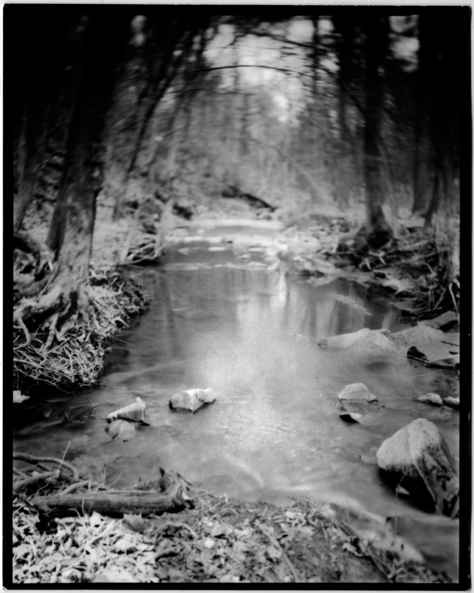
\includegraphics[width=0.4\textwidth]{./img/the_river_10.png}
		\label{fig:PFinput}%
	}
	\hfill
	\subfloat[The Output Image]{%
		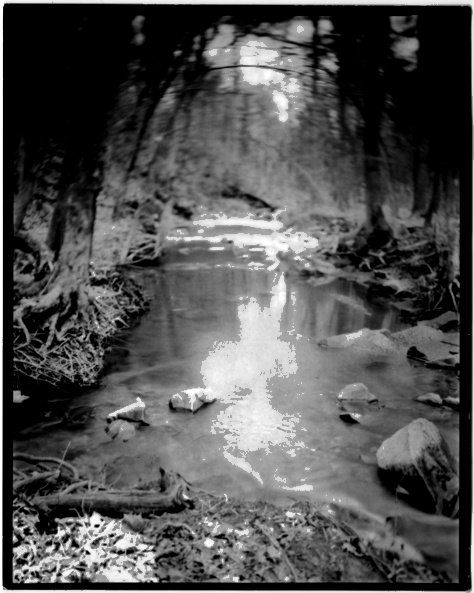
\includegraphics[width=0.4\textwidth]{./img/output.png}
		\label{fig:PFoutput}%
	}
	\hfill
	\caption{Examples a representation of a simple point operation where $O_{ij} = (I_{ij})+20$}
	\label{fig:pointFunction}
\end{figure}
\subsection{Point Operators}
\simpleparagraph{}
Typically the simplest operation in image processing, point operators, deal with pixel transformations also known as a \textbf{point process}\label{point process}. The output image at each pixel depends only on the corresponding input pixel data. This means that, for an input image $I$ and output image $O$ of size $m\times n$ where $I_{ij}$ is a pixel location,
\begin{equation}\label{equ:PToper}
	O_{ij} = a(I_{ij})+b
\end{equation}

\begin{figure}
    \subfloat[The Input Image]{%
	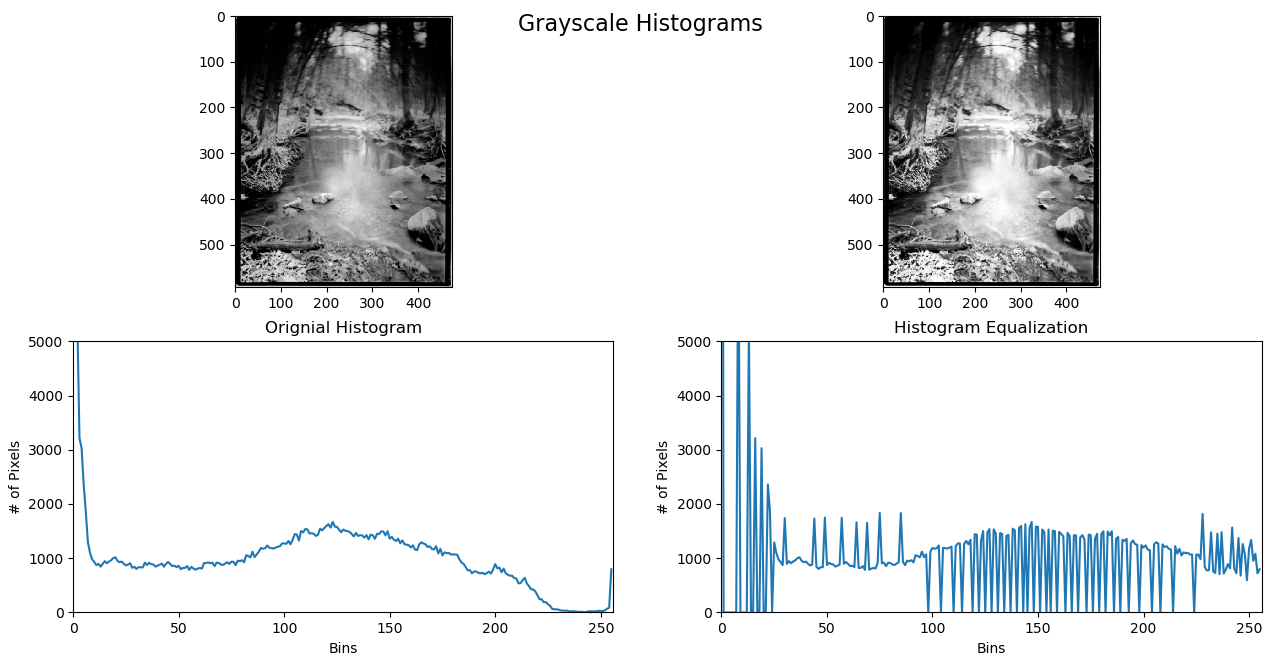
\includegraphics[width=1\textwidth]{./img/Histogram_Equalization.png}
		\label{fig:histrEqu}
	}
	\hfill
	\caption{Histogram Equalization produces a far smoother contrast effect compared to Fig. \ref{fig:pointFunction} above.}
	\label{fig:histrEquTxt}
\end{figure}
represents a general form for a pixel transformation. This assumes that $a>0$ and $\forall a,b \in \mathbb{R}$. The value $a$ is called the \textit{gain} and b is \textit{bias}. In other words, to increase brightness, one would increase the \textit{bias} and to increase the contrast (see Fig. \ref{fig:pointFunction}), one would increase the \textit{gain}.

\subsection{Histograms}
\simpleparagraph{}
Visualizing the changes in image data or representing it in a more compact fashion can be accomplished by forming a distribution like a histogram. The idea of a distribution is to represent how the color values are distributed across an image. For instance, the pixel value 200 red might have 1000 pixels containing that color. Histograms also allow for more dynamic transformations of various pixel data. This means that instead of increasing the image contrast with the point function, use a histogram of pixel values ranging from [0 - 256] (RGB) for each color channel (see Fig. \ref{fig:histrEquTxt}). This is done using a form of the general \textbf{image processing operator}: 
\begin{equation}\label{equ:ProcOper}
g(x,y)=h(f(x,y))\text{\hspace{1cm}or\hspace{1cm}}g(x,y)=h(f_{0}(x,y),\dots,f_{n}(x,y))
\end{equation}
\paragraph[Cumulative Distribution]{}
Notice in Figure \ref{fig:pointFunction}, there are a large amount of artifacts \cite{contributors_distortion_2018} that are produced by the contrast point operation (\ref{equ:PToper}). To make the contrast operation smoother, sum the histograms in the range $0\leq I$ for each $I$\textsuperscript{th} bin of 256 bins. Imagine calculating the grades of a 500 student class; it is much simpler to represent the percent valued grades of each student as a letter grade associated with a group of students. The ``grades" are then used to transform and describe the original image. This will form a \textbf{cumulative distribution} $c(I)$ from the histograms $h(I)$ that will be rescaled and mapped back to the image. Equation \ref{equ:CumulativeDistribution} is the contrast operation and equation \ref{equ:LinearBlend} is the mapping function, also known as a linear blend function where $f(I)$ is the output image.
\begin{align}
c(I) &= \frac{1}{N} \sum_{j=0}^{I} h(i) = c(I-1) + \frac{1}{N}h(I) \label{equ:CumulativeDistribution} \\
f(I) &= \sigma c(I) + (1- \sigma) \label{equ:LinearBlend}
\end{align}
This means that applying gain to each pixel intensity is more spatially\footnote{means occupying space or characterized by space} dynamic and non-linear.
\simpleparagraph{}
Transitioning from using a contrast point function to cumulative distribution is similar to moving from graphing a linear equation like $f(x)=2x+1$ to graphing $f(x)=\int(\sum_{k=0}^{x}ak+b)dx)$. Formally this process is known as a \hyperref[fig:histrEquTxt]{\textbf{histogram equalization}} or CLASHE \cite{pizer_adaptive_1987}, and it will be seen later that gradients involve a similar process. A variant of histogram equalization is used in a popular object recognition technique called SIFT \cite[Lowe 2004]{lowe_distinctive_2004} or Scale Invariant Feature Transforms.

\begin{figure}
	\centering
	\subfloat[Adaptive Histogram Equalization]{%
		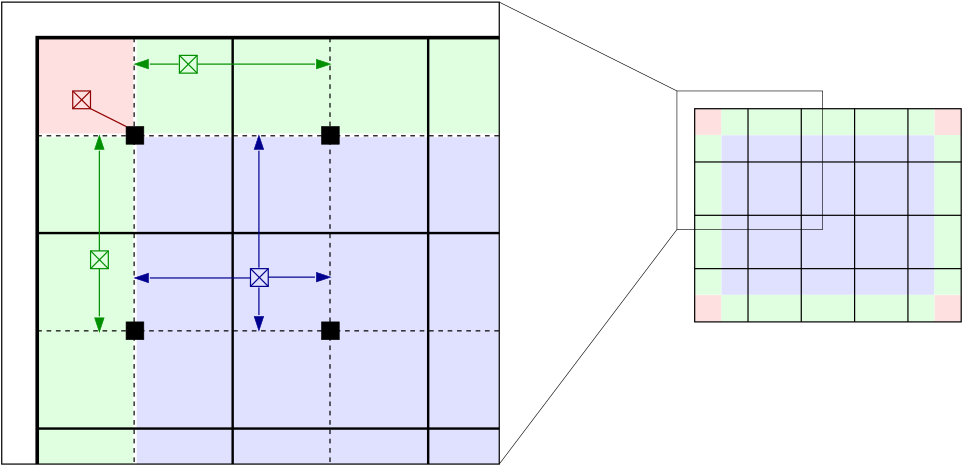
\includegraphics[width=.6\textwidth]{./img/Clahe-tileinterpol.png}
	}
	\hfill
	\caption{The value of the center pixel ($\boxtimes$) is interpolated or formulated from the four black squares ($\blacksquare$).}
	\label{fig:CLASHTileInterpolation}
\end{figure}

\subsection{Filters}
\simpleparagraph{}
Instead of using \textit{global} image information such as a histogram of the color channel distribution, the goal of image filters is to apply some operation locally to a patch of pixel values in an image. For example, image filters can be weighted combinations of pixels in small neighborhoods shown in Figure \ref{fig:CLASHTileInterpolation}. All image filters include some form of \textbf{kernel operation}. To understand what kernels are there a few fundamental linear algebra concepts that need to be covered.

\subsubsection{Linear Systems}
\simpleparagraph{}
Matrices can also be a form of a linear system, $a_{1}x_{1}+a_{2}x_{2}+...+a_{n}x_{n}$ that allows for more efficient solutions. For example, provided the following linear system, find all the variables that solve the equation correctly:
{ \small
	\begin{align*}
	x+2y+3z &= 6\\
	2x-3y+2z &= 14\\
	3x+y-z   &= -2
	\end{align*}
}
It is possible to solve this equation with the \textit{method of elimination} \cite{_elimination_2011}, that is eliminating some variables by adding one equation to another. There is a better way to solve this problem, by representing the equation as a matrix:
{ \small
	\begin{equation}
	A_{coefficients} = \begin{bmatrix}
	1 & 2 & 3 \\
	2 & -3& 2 \\
	3 &  1& -1 
	\end{bmatrix}
	\hspace{5pt}
	x_{variables} = \begin{bmatrix}
	x \\
	y \\
	z \\
	\end{bmatrix}
	b_{solution} = \begin{bmatrix}
	6 \\
	14 \\
	-2 \\
	\end{bmatrix}
	\end{equation}
}
The goal remains the same, find the value of one of the variables. Instead of using the \textit{method of elimination}, transform the coefficient matrix $A$ into a Row Echelon Form \cite{weisstein_echelon_2018}:
{ \small
	\begin{equation}
	REF \begin{pmatrix}
	\begin{bmatrix}[ccc|c]
	1 & 2 & 3 & 6\\
	2 &-3 & 2 & 14\\
	3 & 1 &-1 &-2
	\end{bmatrix}
	\end{pmatrix}
	=
	\begin{bmatrix}[ccc|c]
	1 & 0 & 0 & 1 \\
	0 & 1 & 0 & -2 \\
	0 & 0 & 1 & 3 
	\end{bmatrix}
	=
	\hspace{10pt}
	\begin{matrix}
		1x + 0y + 0z &= \hspace{8pt}1\\
		0x + 1y + 0z &= -2\\
		0x + 0y + 1z &= \hspace{8pt}3
	\end{matrix}
	\end{equation}
}
As shown above, it is possible to solve the linear system using a Row Echelon matrix. Later this matrix transformation will be used to help compute a kernel.

\subsubsection{Matrix Transformations}
\simpleparagraph{}
A Matrix in its most basic form is a rectangular array of size $mn$ with $m$ horizontal rows and $n$ vertical columns. Likewise an image can be thought of as a pixel matrix of size $mn$, and typically a pixel can also be though of as a matrix of size $1\times n$ since it often contains some three-channel 8-bit color data. A matrix of size $1\times n$ or $n\times 1$ is called a vector and can be used to find magnitude and direction. Vectors are used in various applications such as multi-variable calculus or linear algebra. The following are two good visualizations of a vector.
\begin{figure}[h]
	\centering
	\begin{minipage}[a]{0.5\textwidth}
		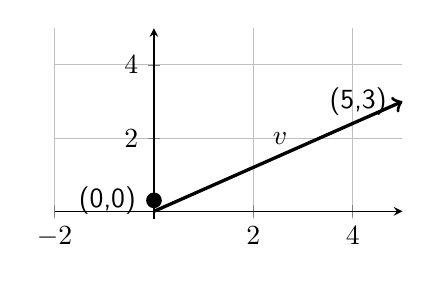
\begin{tikzpicture}
		\begin{axis}[axis lines=middle,grid=both, width=6cm,height=4cm, xmin=-2,xmax=5, ymin=-.2,ymax=5]
		\coordinate (A) at (axis cs: {0}, {0});
		\coordinate (B) at (axis cs: {5}, {3});
		\draw[very thick,->](A)--(B);
		\node[label={180:{(0,0)}},circle,fill,inner sep=2pt] at (axis cs:0,0.3) {};
		\node[label={180:{(5,3)}},inner sep=2pt] at (axis cs:5,3) {};
		\node[label={180:{$v$}},inner sep=2pt] at (axis cs:3,2) {};
		\end{axis}
		\end{tikzpicture}
	\end{minipage}
	\hfill
	\begin{minipage}[b]{0.4\textwidth}
		\centering
		{\large
			$v = 
			\begin{bmatrix}
			5 \\
			3 \\
			\end{bmatrix}$
		}
	\end{minipage}
	\hfill
	\caption{Example of a (a) Cartesian and (b) matrix form of a vector.}
	\label{equ:basicVector}
\end{figure}
\paragraph[Road-Map]{}
Matrices and vectors are not simply a different notation of representing numbers, but contain powerful and unique properties and operations. For example, the traveling salesman problem can be solved by the Hungarian Method in $O(n^{3})$ time \cite{baripada_college_hungarian_2017}. This is done using a matrix that represents the costs and performs various matrix transformations to reliably solve the problem. Scalar multiplication and addition, transposition, and inverses are the basic matrix transformations and building blocks for geometric transformations. Likewise, finding the direction and magnitude of a vector is vital to understanding HOG and other feature descriptors.

\paragraph[Scalars]{} A \textbf{scalar} is a single real number that is scaled to appropriate units of measure \cite{larson_calculus_2014}. In other words, a scalar is used to resize an image or change the pixel values of the overall image like in the contrast point process \eqref{equ:PToper}. Applying a scalar to a matrix would operate as follows:
{ \small
	\begin{equation}\label{equ:ScalarMultiplication}
	3
	\begin{bmatrix}
	2 & 1 \\
	5 & 3
	\end{bmatrix}
	=	
	\begin{bmatrix}
	6  & 3 \\
	15 & 9
	\end{bmatrix}
	\end{equation}
}
\paragraph[Transpose]{} Denoted by the symbol $A^{T}$ where $A$ is any matrix, the \textbf{transpose} of the matrix will interchange the rows and columns of $A$, implying that $a^{T}_{ij}=a_{ji}$. The properties of transpose allow for more complex problems to be solved, such as matrix multiplication.
{ \small
	\begin{equation}\label{equ:Transpose}
	A =
	\begin{bmatrix}
	a_{11} & a_{12} & a_{13}\\
	a_{21} & a_{22} & a_{23}
	\end{bmatrix}
	,
	A^{T}=
	\begin{bmatrix}
	a_{11} & a_{21} \\
	a_{12} & a_{22} \\
	a_{13} & a_{23}
	\end{bmatrix}
	\end{equation}
}
\paragraph[Matrix Multiplication]{} Instead of multiplying a single value to a matrix, it also possible to multiply matrices together, also known as a \textbf{matrix multiplication}. This is done by multiplying two matrices, $A=[a_{ij}]$ of size $m\times p$ and $B=[b_{ij}]^{T}$ of size $p\times n$.
{ \small
	\begin{align*}
	A&=
	\begin{bmatrix}
	1 & 2 & -1\\
	3 & 1 & 4
	\end{bmatrix}
	,\hspace{3pt}
	B=
	\begin{bmatrix}
	-2 & 5 \\
	4 & -3 \\
	2 & 1
	\end{bmatrix}
	\end{align*}
	\begin{align*}
	\sum_{k=1}^{p}a_{ik}a_{jk},\hspace{3pt}
	A\times B &=
	\begin{bmatrix}
	(1)(-2)+(2)(4)+(-1)(2) & (1)(5)+(2)(-3)+(-1)(1)\\
	(3)(-2)+(1)(4)+(4)(2) & (3)(5)+(1)(-3)+(4)(1)
	\end{bmatrix}
	\\
	&=
	\begin{bmatrix}
	4 & -2\\
	6 & 16
	\end{bmatrix} \numberthis \label{equ:MatrixMultiplication}
	\end{align*}
}
\paragraph[Inverse]{} The \textbf{inverse} of a matrix is a powerful tool for forming a wide variety of both color and geometric changes. A matrix $A$ of size $n\times n$ is invertible if there is some matrix $A^{-1}$ that $AA^{-1}=I_{n}$. The matrix $I_{n}$ is an identity matrix, which is a matrix of 1's on the diagonal $I_{ii}, (0 \leq i \leq n)$ and 0's everywhere else.
{ \small
	\begin{equation}\label{equ:IdentityMatrix}
	I_{n}
	\begin{bmatrix}
	1 		& 0 	& \dots	 & 0 \\
	0 		& 1 	& \dots	 & 0 \\
	\vdots 	& \vdots& \ddots & \vdots \\
	0		& 0		& \dots  & 1
	\end{bmatrix}
	\end{equation}
}
Therefore the inverse would be found by obtaining a linear system and finding values that will satisfy the definition of an inverse.
{ \small
	\begin{equation}\label{equ:InverseMatrix}
	A=
	\begin{bmatrix}
	1 & 2\\
	3 & 4 
	\end{bmatrix}
	,\hspace{1cm}
	A^{-1}=
	\begin{bmatrix}
	a & b\\
	c & d 
	\end{bmatrix}
	\end{equation}
}
Solve
{ \small
	\begin{equation}\label{equ:InverseMatrixSolved}
	AA^{-1}=
	\begin{bmatrix}
	a+2c & b+2d\\
	3a+4c & 3b+4d
	\end{bmatrix}
	=
	\begin{bmatrix}
	1 & 0\\
	0 & 1 
	\end{bmatrix}
	\end{equation}
	\begin{align*}
	A^{-1}=
	\begin{bmatrix}
	-2 & 1\\
	\frac{3}{2} & -\frac{1}{2}
	\end{bmatrix}
	\end{align*}
}
\paragraph[Magnitude \& Direction]{Magnitude \& Direction}
Suppose that a vector $\textbf{v}$ with two elements represents the x and y points on a graph. How could one find the length of $\textbf{v}$ in the graph \eqref{equ:basicVector}? Simple, since the x and y elements of the vector form a triangle, use Pythagorean theorem to find it:
\begin{equation}\label{equ:VectorNorm}
	\norm{\textbf{v}}=\sqrt{v_{x}^{2}+v_{y}^{2}}
\end{equation}
In computer vision this is called the \textbf{normal} or \textbf{magnitude} of a vector, since the length of $\textbf{v}$ is also the measure of change from the origin to the point. Since there are two points to measure, the y-axis ($\textbf{u}=[0,y]$) and the vector elements ($\textbf{v}=[5,3]$), it is possible to find the direction of line:
\begin{equation}\label{equ:VectorDirection}
cos\theta = \frac{u_{1}v_{1}+u_{2}v_{2}}{\norm{\textbf{u}}\norm{\textbf{v}}}
\end{equation}
In this case it the magnitude of $\norm{\textbf{v}}$ is 5.83\dots and the direction is $~49^{o}$. The value $y\neq0$ can be any real number and cannot impact the direction formula. The norm can be used to convert the values of $\textbf{v}$ to be in the range [0-1]. For example:
{ \small
	\begin{equation}\label{equ:L2Norm}
	\begin{bmatrix}
	\frac{5}{5.83\dots}\\
	\frac{3}{5.83\dots}
	\end{bmatrix}
	\hspace{.2cm}
	=
	\hspace{.2cm}
	\begin{bmatrix}
	0.8574\dots\\
	0.5144\dots
	\end{bmatrix}
	\end{equation}
}

\subsubsection{Geometric Transformations}
\simpleparagraph{}
Using the concepts of matrix transformations, it is possible to alter the geometric properties of a matrix. In preprocessing, it is used to allow for more robust feature matching. SIFT or Scale Invariant Feature Transforms \cite{lowe_distinctive_2004} produce features that are geometrically invariant of affine changes. Before the term affine is defined; reflections, rotations, shears, scale, and translations must be reviewed. All the transformations will be operated on the following triangle formed by the points $(-1, 4)$, $(3, 1)$, and $(2, 6)$.
\begin{figure}[h]
	\centering
	\begin{minipage}[Cartesian Form]{0.5\textwidth}
		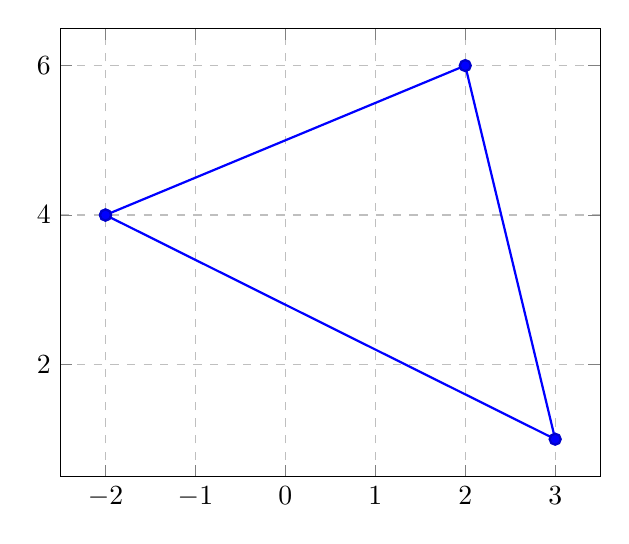
\begin{tikzpicture}
		\begin{axis}[
		scatter, % To colour the points
		point meta=explicit, % To be able to specify the column for the colours
		shader=flat corner, % To use the color of one point for the line segment
		ymajorgrids=true, % Adds grid Y lines
		xmajorgrids=true, % Adds grid X lines
		grid style=dashed
		]
		\addplot [
		mesh,   % Colour the lines
		thick
		] table [meta=phase] {
			time value phase
			-2 4 1
			3 1 1
			2 6 1
			-2 4 1
		};
		\end{axis}
		\end{tikzpicture}
	\end{minipage}
	\hfill
	\begin{minipage}[Matrix Form]{0.4\textwidth}
		\centering
		{\large
			$\begin{bmatrix}[c|c|c]
				-1 & 3 & 2\\
				4 & 1 & 6
			\end{bmatrix}$
		}
	\end{minipage}
	\hfill
	\caption{Example triangle (a) formed by the matrix (b) that is used for the subsequent Geometric transformations.}
	\label{fig:Triangle}
\end{figure}


\paragraph[Reflection]{} The Reflection of a matrix with respect to the x-axis or y-axis is a matrix-vector product of an diagonal matrix and a n-dimensional point. In matrix multiplication, the second matrix was transposed to multiply each element row by row. With the matrix-vector product, it will produce a vector that has been \textit{scaled} by a vector with the initial matrix. In the case of reflection, the following matrices will rotate vectors' values with respect to the x or y axis:
{ \small
	\begin{equation}\label{equ:XReflection}
	A=
		\begin{bmatrix}
		1 & 0\\
		0 & -1 
		\end{bmatrix}
	\textbf{v}_{x-axis}=
		\begin{bmatrix}
		x\\
		y
		\end{bmatrix}
	=	
		\begin{bmatrix}
		x\\
		-y
		\end{bmatrix}
	,
		\hspace{1cm}
		\begin{bmatrix}
		1 & 0\\
		0 & -1 
		\end{bmatrix}
		\begin{bmatrix}[c|c|c]
		-1 & 3 & 2\\
		4 & 1 & 6
		\end{bmatrix}
	=
		\begin{bmatrix}[c|c|c]
		-1 &  3 &  2\\
		-4 & -1 & -6
		\end{bmatrix}
\end{equation}
\begin{equation}\label{equ:YReflection}
	A=
		\begin{bmatrix}
		0 & -1\\
		-1 & 0 
		\end{bmatrix}
	\textbf{v}_{y-axis}=
		\begin{bmatrix}
		x\\
		y
		\end{bmatrix}
	=	
		\begin{bmatrix}
		-y\\
		-x
		\end{bmatrix}
	,
		\hspace{1cm}
		\begin{bmatrix}
		 0 &-1\\
		-1 & 0
		\end{bmatrix}
		\begin{bmatrix}[c|c|c]
		-1 & 3 & 2\\
		4 & 1 & 6
		\end{bmatrix}
	=
		\begin{bmatrix}[c|c|c]
		-4 & -1 & -6\\
		 1 & -3 & -2
		\end{bmatrix}
	\end{equation}
}
%MAYBE Include graph representation.

\paragraph[Rotations]{} Similar to reflections, \textbf{rotations} are also a matrix-vector product with one important difference, the matrix is a composed of sines and cosines with an arbitrary angle $\theta$. For example, where $\theta = 90^{o}$
{\small 
\begin{equation}\label{equ:Rotation}
	\centering
	A\textbf{v}=
	\begin{bmatrix}
	cos\theta & -sin\theta\\
	sin\theta & cos\theta 
	\end{bmatrix}
	\begin{bmatrix}[c|c|c]
	-1 & 3 & 2\\
	4 & 1 & 6
	\end{bmatrix}
	=
	\begin{bmatrix}[c|c|c]
	-4 & -1 & -6\\
	-1 &  3 &  2
	\end{bmatrix}
	\end{equation}
}
\paragraph[Shears]{}Unlike a reflection or rotation, which maintain the \textit{shape} of the object formed by the three points, \textbf{shears} allow for the transformation of one direction. This is quite useful for correcting misaligned objects within an image, which can dramatically decrease the FPPW (False Positives per Window). The scalar $k$ can be any real number, and tends to be either the $cot\theta$ or some constant. In this case, $k=cot(10)$:
{\small 
	\begin{equation}\label{equ:Shears}
	\centering
	A\textbf{v}=
	\begin{bmatrix}
	1 & k\\
	0 & 1 
	\end{bmatrix}
	\begin{bmatrix}[c|c|c]
	-1 & 3 & 2\\
	4 & 1 & 6
	\end{bmatrix}
	=
	\begin{bmatrix}[c|c|c]
	~5.2 & ~4.5 & ~11.3\\
	4 &  3 &  2
	\end{bmatrix}
	\end{equation}
}
Notice how the second row, the y-axis, was unaffected by the shear operator.

\paragraph[Scale]{} \textbf{Scaling} a matrix is one of the simplest geometric operations, it essentially applies a scalar to the x and y values respectively. Therefore, if one wanted to scale the triangle in Figure \ref{fig:Triangle} to be double its size, simply apply the following formula with $\beta=[2,2]$:
{\small 
	\begin{equation}\label{equ:Scale}
	\centering
	A\textbf{v}=
	\begin{bmatrix}
	\beta_{x} & 0\\
	0 & \beta_{y} 
	\end{bmatrix}
	\begin{bmatrix}[c|c|c]
	-1 & 3 & 2\\
	 4 & 2 & 6
	\end{bmatrix}
	=
	\begin{bmatrix}[c|c|c]
	-2 & 6 & 4\\
	 8 & 2 & 12
	\end{bmatrix}
	\end{equation}
}

\paragraph[Translations]{} Up to this point, all of the transformations have been scalar based, but it is also possible to perform vector-addition to move the triangle around the plane. Suppose that one wanted to displace or move the points of the triangle to the right, simply add some constant $\sigma=[2,0]$ to each element in the point. This is also known as \textbf{translation}.
{\small 
	\begin{equation}\label{equ:Translation}
	\centering
	T=
	\begin{bmatrix}
	\sigma_{x}\\
	\sigma_{y}
	\end{bmatrix}
	+
	\begin{bmatrix}[c|c|c]
	-1 & 3 & 2\\
	 4 & 2 & 6
	\end{bmatrix}
	=
	\begin{bmatrix}[c|c|c]
	1 & 5 & 4\\
	4 & 2 & 6
	\end{bmatrix}
	\end{equation}
}
\paragraph[Affine Transforms]{}
Notice that all of these transformations are dealing with x and y points on a Cartesian Plane. This means that all of the transformations are spatial or in space. This is exactly what the term affine defines, it is an extension of a vector space that includes an additional type of object, the point. Therefore, when papers like \cite[Distinctive Image Features from Scale-Invariant Keypoints][]{lowe_distinctive_2004} describes its features as scale and affine invariant, it means that the features do not vary spatially. This is why SIFT was often used in moving scenes for large objects.

\subsubsection{Vector Spaces}
\simpleparagraph{}
Another integral component to a kernel is a vector space, which are defined as a set of objects and two operations $\oplus$ and $\odot$ on these objects \cite{weisstein_vector_2018}. The set of objects in this case are a set of vectors denoted as $R^{n}$\footnote{$R^{n}$ is the set of $n\times 1$, column matrices, $R_{n}$ is the set of $n\times 1$, row matrices, and $M^{mn}$ is set of $m\times n$ matrices} with each vector of size $n$. Now to understand what the operations $\oplus$ and $\odot$ do starting with $\oplus$, suppose there are two $1\times n$ matrices where $\oplus$ is denoted as a sum operator or \textbf{vector addition}:
{ \small
\begin{equation}
	\begin{bmatrix}
	a_{1} & a_{2} & \dots & a_{n}
	\end{bmatrix}
	\oplus
	\begin{bmatrix}
	b_{1} & b_{2} & \dots & b_{n}
	\end{bmatrix}
	=
	\begin{bmatrix}
	a_{1}+b_{1} & a_{2}+b_{2} & \dots & a_{n}+b_{n}
	\end{bmatrix}
\end{equation}
}
The multiplication operator $\odot$ or \textbf{scalar multiplication} works the same way:
{ \small
\begin{equation}
	A
	\begin{bmatrix}
	a_{11} & a_{12} & a_{13}\\
	a_{21} & a_{22} & a_{23}\\
	a_{31} & a_{32} & a_{33}
	\end{bmatrix}
	\odot
	B
	\begin{bmatrix}
	b_{11} & b_{12} & b_{13}\\
	b_{21} & b_{22} & b_{23}\\
	b_{31} & b_{32} & b_{33}
	\end{bmatrix}
	=
	\begin{bmatrix}
	a_{11}b_{11} & a_{12}b_{12} & a_{13}b_{13}\\
	a_{21}b_{21} & a_{22}b_{22} & a_{13}b_{13}\\
	a_{31}b_{31} & a_{32}b_{32} & a_{33}b_{33}
	\end{bmatrix}
\end{equation}
}
The resulting matrix would thus be denoted as a vector space of $M_{33}$. Using the properties of a matrix and vectors and operations of a vector space, it is possible to perform a kernel operation. Now sum the scalar multiplier ($A\odot C$) and plug in values some pixel values into $A$ and an edge detection kernel into $B$.
{ \small
\begin{equation}\label{equ:matrixKernelSetup}
	A=
	\begin{bmatrix}
	158 & 249 & 125\\
	211 & 227 & 114\\
	178 & 246 & 123
	\end{bmatrix}
	\text{\hspace{5pt}and\hspace{5pt}}
	B=
	\begin{bmatrix}
	-1 & -1 & 1 \\
	-1 &  8 & 1 \\
	-1 & -1 & 1
	\end{bmatrix}
\end{equation}
}
C is defined as $B=R(R(B)^T)^T$. This produces the effect of swapping the rows and columns by rotating the transposition of the rotation of $B^T$, which looks like so:
{ \small
	\begin{equation}\label{equ:matrixKernelRotate}
	\begin{bmatrix}
	a_{11} & a_{12} & a_{13}\\
	a_{21} & a_{22} & a_{23}\\
	a_{31} & a_{32} & a_{33}
	\end{bmatrix}
	=
	\begin{bmatrix}
	a_{33} & a_{32} & a_{31}\\
	a_{23} & a_{22} & a_{21}\\
	a_{13} & a_{12} & a_{11}
	\end{bmatrix}
	\end{equation}
}
Now perform the kernel operation:
{ \small
	\begin{align*}
	\sum A\odot C &=	(a_{11}b_{33}) + (a_{12}b_{32}) + (a_{13}b_{31}) + (a_{21}b_{23}) + (a_{22}b_{22}) + (a_{13}b_{21})\\
				  &+ (a_{31}b_{13}) + (a_{32}b_{12}) + (a_{33}b_{11})\\
			  	  &= (158\cdotp -1)+(249\cdotp -1)+(125\cdotp -1) + (211\cdotp -1)+(227\cdotp 8)+(114\cdotp -1)\\
			  	  &+ (178\cdotp -1)+(246\cdotp -1)+(123\cdotp -1)\\
			  	  &=  412 \numberthis \label{equ:matrixKernelSolve}
	\end{align*}
}
There is a problem, the output is too large to be considered a pixel value and therefore it is necessary to normalize by dividing the output by the sum of the kernel matrix. This operation of summing the scalar multiplication of two vector spaces is more widely known as a \textbf{kernel convolution} (denoted by the symbol $*$ or $\otimes$). The resulting value that has been normalized is the value of the center pixel, $a_{22}$. When implemented, a kernel convolution follows the following formula, where $s$ is the size of the kernel matrix:
\begin{equation}\label{equ:ConvolutionKernel}
	O[i,j]= \sum_{l=-s}^{s}\sum_{k=-s}^{s} I[u,v]K[i-l,j-k]
\end{equation}
Sometimes it is easier to understand a convolution by its discrete operator above or its matrix operator in the equations \ref{equ:matrixKernelSetup}, \ref{equ:matrixKernelRotate}, \ref{equ:matrixKernelSolve}. Another type of kernel operation that is also often used in image processing is called \textbf{Cross-Correlation} (also denoted by the symbol $\otimes$ - pay attention to the discrete forms) and is simply the sum of the scalar multiplier ($A\odot B$) where B is not flipped. In discrete form it looks like so:
\begin{equation}\label{equ:CrossCorrelationKernel}
O[i,j]= \sum_{l=-s}^{s}\sum_{k=-s}^{s} I[u,v]K[i+l,j+k]
\end{equation}

\subsection{Gradients}
\simpleparagraph{}
Unlike a simple edge detection kernel shown in equation \ref{equ:ConvolutionKernel}, gradients allow for more complex kernel operations that are formed by a non-linear equation. The gradient equation will take in a pixel value at $i$ and $j$ for all pixels in an image and produce an image that represents the change of the image with respect to both $x$ and $y$ of the image function $f(x,y)$. The formal definition of a gradient is a partial derivative of a vector-valued function of two variables:
{ \small
	\begin{equation}\label{equ:gradientFunction1}
	\nabla F(x,y)=f_{x}(x,y)\textbf{i}+f_{y}(x,y)\textbf{j}
	\end{equation}
	\begin{equation}\label{equ:gradientFunction2}
	\nabla F=
		\begin{bmatrix}
		\frac{\partial F}{\partial x} & \frac{\partial F}{\partial y}
		\end{bmatrix}
	\end{equation}
}
The two equations represent the same gradient operation in two forms. The first is in the form of a vector-valued function\footnote{The concept of a vector-valued function is functionally the same as an affine transformation.} that will produce the gradient vector $\begin{bmatrix}f_{x}(x,y) & f_{y}(x,y)\end{bmatrix}$. Therefore, to be able to understand and compute this formula, it is necessary to briefly introduce the concept of partial derivatives.

\subsubsection{Partial Derivatives}
\simpleparagraph{}
In Calculus, finding a derivative is in essence finding the tangent of a line. A tangent is simply the slope or rate of change at a point in space for some function. An affine vector is also the measure of direction \eqref{equ:VectorDirection} and magnitude \eqref{equ:VectorNorm} in space that is transformed by some system of linear equations. Finding the slope for all the linear equations formed by the affine matrix is also known as a \textbf{partial derivative}. This means that for the function $f(x,y)=x^{2}y+sin(y)$ at the point $(1,2)$,
{ \small
\begin{align*} 
	\frac{\partial f}{\partial x}(x,y) &\Longrightarrow \frac{\partial f}{\partial x}(x^{2}y+sin(y)) \Longrightarrow f_{x}(x,y) = 2xy+0\\
	f_{x}(1,2)&=4\\
	\end{align*} 
	\begin{align*} 
	\frac{\partial f}{\partial y}(x,y) &\Longrightarrow \frac{\partial f}{\partial y}(1^{2}y+cos(y)) \Longrightarrow f_{y}(x,y) = x^{2}+cos(y)\\
	f_{y}(1,2)&=0.5838\dots \numberthis \label{equ:SimplePartialDerivative} \\
\end{align*}
}
Now that the partial derivatives has been computed, put $f_{x}(1,2)$ and $f_{y}(1,2)$ back into the form of equation \ref{equ:gradientFunction1}:
\begin{equation}\label{equ:SimpleGradient}
	\nabla f(1,2)=4\textbf{i}+0.5838\textbf{j}\\
	\nabla f(1,2)=4.5838
\end{equation}

\begin{figure}[h]
	\centering
	\subfloat[2-D Distribution]{%
		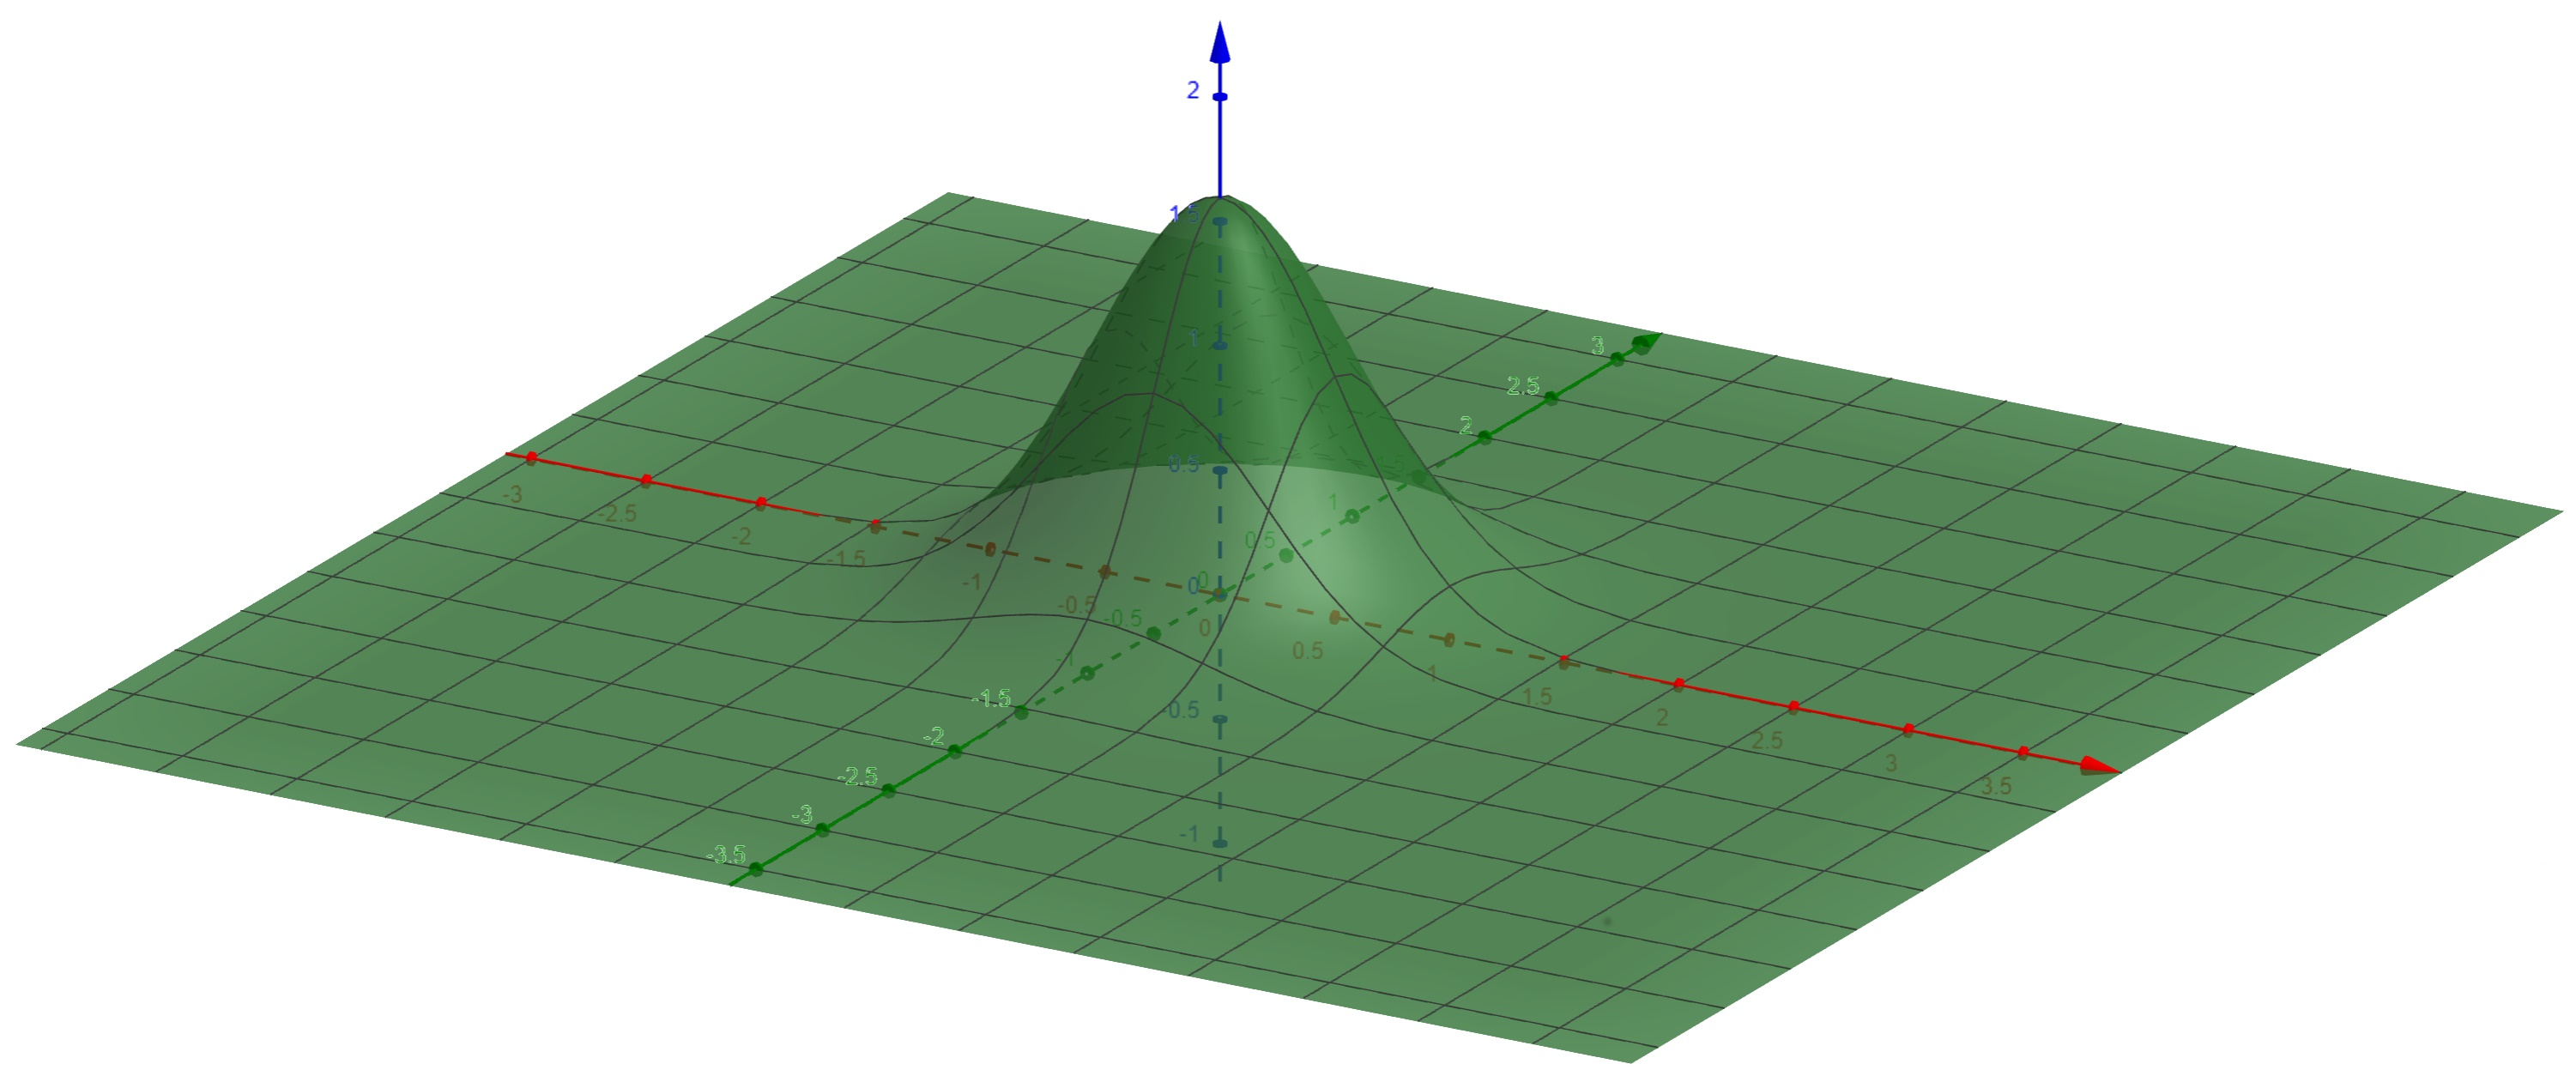
\includegraphics[width=0.4\textwidth]{./img/Gradient2D.png}
		\label{fig:GradientDistribution}%
	}
	\hfill
	\subfloat[Gausian Kernel]{%
		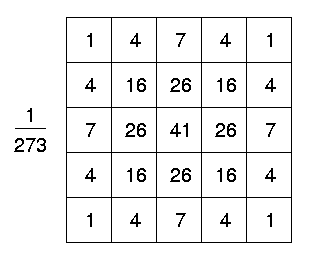
\includegraphics[width=0.3\textwidth]{./img/gausmask.png}
		\label{fig:GaussianMask}%
	}
	\hfill
	\caption{Example of a 2-D Gradient Distribution that forms a Gaussian Convolution Kernel, 273 is the sum of all the values in the kernel filter}
	\label{fig:GaussianSmoothing}
\end{figure}

\subsubsection{Calculation}
\simpleparagraph{}
Now that the concept of partial derivatives has been covered, it is possible to form a gradient image. Since the gradient produces a vector at each pixel, it can be used to also form a convolution kernel with some predetermined values. The convolution kernel produced by the gradient function
{\small 
	\begin{equation}\label{equ:GaussianSmoothing}
	G(x,y)=\frac{1}{2\pi \sigma^{2}}e^{-\frac{x^{2}+y^{2}}{2\sigma^{2}}}
	\end{equation}
}
where $\sigma$ is some constant smooths the image, is also known as Gaussian Smoothing see Fig. \ref{fig:GaussianSmoothing}. If a white image was given as input, there would be no change at any point in the image and thus the gradient vector for every point or pixel would look like so:
{ \small
	\begin{equation}\label{equ:gradientFunctionBlank}
	\nabla F=
	\begin{bmatrix}
	0 & 0
	\end{bmatrix}
	\end{equation}
}
If there was change only in the $x$ or $y$ direction,
{ \small
	\begin{equation}\label{equ:gradientFunctionXorY}
	\nabla F_{x}=
	\begin{bmatrix}
		\frac{\partial F}{\partial x} & 0
	\end{bmatrix}
	,\hspace{.5cm}
	\nabla F_{y}=
	\begin{bmatrix}
		0 & \frac{\partial F}{\partial y}
	\end{bmatrix}
	\end{equation}
}
Once the gradient has been computed for some pixel $ij$ in the image, it is possible to find the direction \eqref{equ:GradientDirection} and magnitude \eqref{equ:GradientMagnitude} of the gradient vector using the following formulas:
{\small
	\begin{equation}\label{equ:GradientDirection}
		\theta = tan^{-1}
		\begin{pmatrix}
			\frac{\partial F}{\partial x} &/& \frac{\partial F}{\partial y}
		\end{pmatrix}
	\end{equation}
	\begin{equation}\label{equ:GradientMagnitude}
	\norm{\nabla F} = 
		\sqrt{(\frac{\partial F}{\partial x})^{2} + (\frac{\partial F}{\partial y})^{2}}
	\end{equation}
}

\begin{figure}[h]
	\centering
	\subfloat[Image Pyramid]{%
		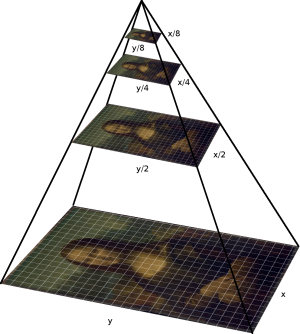
\includegraphics[width=.3\textwidth]{./img/image_pyramid_ex.png}
			\label{fig:ImagePyramidImg}%
	}
	\hfill
	\caption{The traditional image pyramid, where the base is most fine resolution and the top is the most corse. Each level is half the size of the previous.}
	\label{fig:ImagePyramid}%
\end{figure}
\subsection{Image Pyramids}
\simpleparagraph{}
The final key concept necessary to understanding HOG are \textbf{image pyramids}. They are a multi-resolution representation of an image and are used to rescale the image to various sizes for detecting different objects at different scales. Image pyramids find objects at various locations by using a \textbf{sliding window}, which is also called the \textbf{detection window}. Calculating an image pyramid of $n$ levels involves two processes, Gaussian smoothing which was described above (see \ref{fig:GaussianSmoothing}) and sampling. At each level, it stores the differences between the image at that level and the predicted image from the next level.%\ref{wavelets-ppt}

\simpleparagraph{}
The concept of sampling is derived from Wavelets and Fourier Transforms. \textbf{Sampling} is defined as the process of producing a finite set of points from a continuous function that has been derived from an image. Similar to the cumulative distribution in section \ref{subsec:Histograms}, wavelets and Fourier transforms are ordinary multivalued functions of one dimension applied to signals. Wavelets and Fourier transforms have a number of applications, such as audio, signal or image processing. How could an image be a signal? Consider the fact that an image is a collection of two dimensional data points that can be graphed to a Cartesian Plane. Audio signals are the same, yet are a collection of one dimensional data points. As the concept of partial derivatives has shown, $x$ and $y$ can be separated to produce two functions accordingly. Therefore an image is a signal or two signals with the functions $f(x)$ and of $f(y)$.

\simpleparagraph{}
Fourier transforms are only sinusoid or sin wave functions, whereas wavelets have a wide variety of families. Wavelets are also localized in space and therefore are variable at different window sizes; however, Fourier transforms are affine invariant. This implies that wavelets are better suited for recognizing spatially bound objects. Many of the earliest real-time object detectors utilized a special type of wavelet known as a Haar wavelet \cite{viola_rapid_2001}. This framework was later improved upon in SURF or Speeded-Up Robust Features \cite{bay_speeded-up_2008}.

\simpleparagraph{}
When creating an image pyramid, sampling is used to produce an image of either higher or lower\footnote{Oftentimes a higher resolution or size of an object such as an image or histogram is referred to as fine, and inversely coarse for a lower resolution.} resolution, hence the name \textbf{multi-resolution}. The two types of sampling are \textbf{interpolation} or \textit{upsampling}, and \textbf{decimation} or \textit{downsampling}.

\paragraph[Sampling]{}
To sample an image, one must use a wavelet or Fourier transform to produce a convolution kernel that will be plugged into one of the two formulas, either for upsampling \eqref{equ:Upsampling} or downsampling \eqref{equ:Downsampling}.
{\small
\begin{equation}\label{equ:Upsampling}
	O[i,j]= \sum_{l=-s}^{s}\sum_{k=-s}^{s} I[u,v]K[i-rl,j-rk]
\end{equation}
\begin{equation}\label{equ:Downsampling}
	O[i,j]= \sum_{l=-s}^{s}\sum_{k=-s}^{s} I[u,v]K[ri-l,rj-k]
\end{equation}
}
The constant $r$ is the sampling rate. In upsampling it is used to make the kernel deal with a finer scale of pixels, whereas, in downsampling it reduces the scale of the pixels.

\section{HOG Feature Descriptors}
\simpleparagraph{}
Feature Descriptors reflect a major component within the field of computer vision. Various types of feature descriptors are used to analyze, describe, and match images. There are two general types of features, key-point or appearance profiles and edge profiles, and both are some form of affine vector space object. HOG's features are edge based, which are simpler and easier to understand compared to key-point descriptors. There are five general steps to creating HOG features, aimed at evaluating well-normalized local histograms of image gradient orientations in a dense grid.

\subsection{Preprocessing}
\simpleparagraph{}
The first step in the HOG process is to prepare the images to produce the most robust feature set possible. Since there is a lot of unnecessary information and the objects within the image have a unique scale, it is important to filter and form an image pyramid. Typically the initial filters applied to the image are normalized corrections of gamma\footnote{Also known as exposure or overall intensity of an image.} and color. Since the location of the objects are unknown, it is necessary to use a detection window scaled to each level in the pyramid. This window will \textit{crop} the image and describe the features within that sub-image only. The pyramids will then be calculated using Gaussian Smoothing and then downsampled for a number of scales\footnote{Typically 4 or 8 scales are used}.

\subsection{Gradient Images}
\simpleparagraph{}
Once the image has been preprocessed, the gradients can be calculated. There are various types of gradient filters available to use, but for simplicity sake, a 1-D centered filter for both $x$ or $y$ will be employed.
{ \small
	\begin{equation}\label{equ:1DMask}
	\begin{bmatrix}
	-1 & 0 & 1\\
	\end{bmatrix}
	\hspace{1cm}	
	\begin{bmatrix}
	-1\\
	0\\
	1
	\end{bmatrix}
	\end{equation}
}
Two images will be produced, one for the x-gradient image and the y-gradient image. From these two images, the magnitude and direction can be computed and is now ready to be placed in histograms. Not only does the gradient calculation provide the essential data for the features, it will also remove a large amount of unnecessary data.

\begin{figure}
	\subfloat[Oritation Bins]{%
		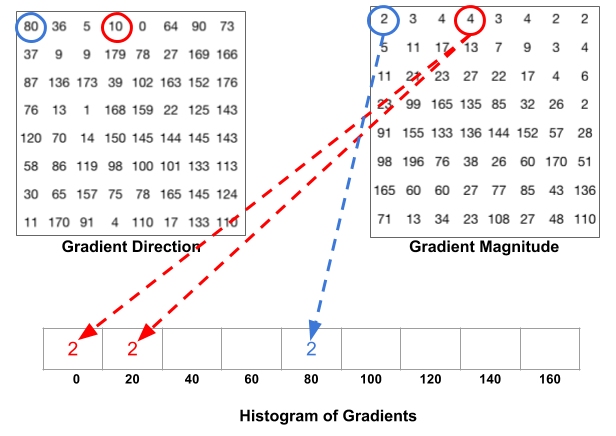
\includegraphics[width=.4\textwidth]{./img/hog-histogram-1}
	}
	\hfill
	\subfloat[8x8 Histogram]{%
		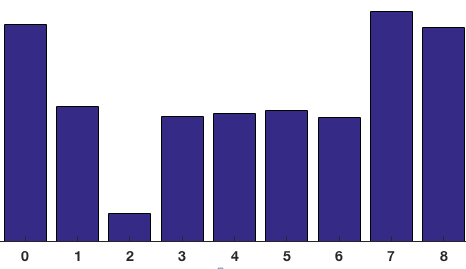
\includegraphics[width=0.4\textwidth]{./img/histogram-8x8-cell}
	}
	\hfill
	\caption{The $9\times 1$ histograms formed by the gradient vectors for a descriptor block \cite{mallick_histogram_2016}.}
	\label{fig:HistrogramBins}
\end{figure}

\subsection{Gradient Histograms}
\simpleparagraph{}
Now that the gradients have been prepared, it is time to place them into histograms. Unlike the histograms of color data in section \ref{subsec:Histograms}, the histogram will be formed with 9 orientation bins of angles $0-180^{o}$ as the x-axis and the sum of the gradient magnitudes as the y-axis. A gradient's direction will denote what direction bin the magnitude will be added to. Notice figure \ref{fig:HistrogramBins}, the 9 bins are given a direction, and if the gradient direction is split between two bins the magnitude will be evenly divided among the two bins.
\simpleparagraph{}
Since each histogram describes a single edge orientation and magnitude, there must be multiple smaller histograms to provide accurate edge features. An object is made up of various edge orientations, and not simply a single edge feature; therefore, the image will split up into blocks, which can be used in various sizes dependent on the object scale. In a $64\times 128$ size detection window, $8\times 8$ blocks are recommended. Inside each block a gradient histogram is calculated.

\begin{figure}[h]
	\centering
	\subfloat[HOG Gradients]{%
		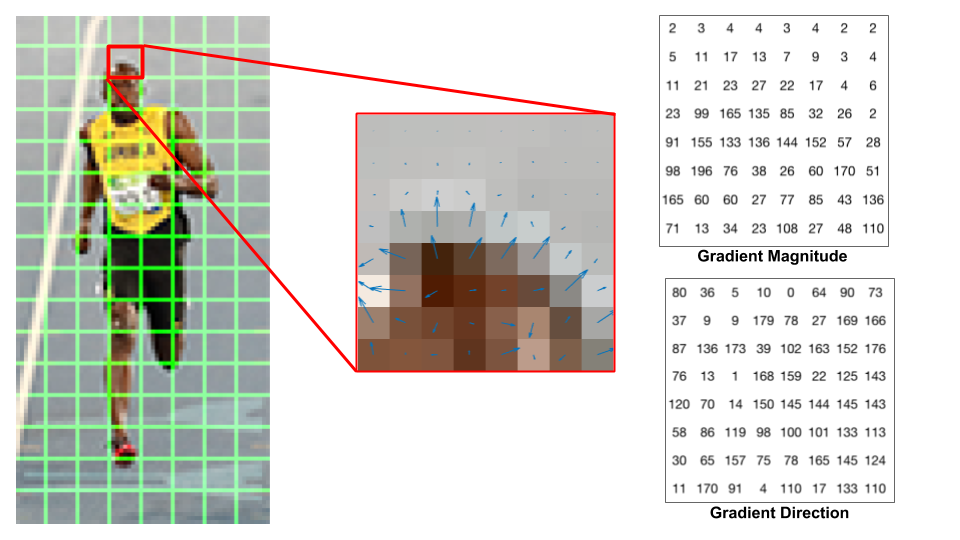
\includegraphics[width=0.5\textwidth]{./img/hog-cell-gradients}
	}
	\hfill
	\subfloat[HOG Blocks]{%
		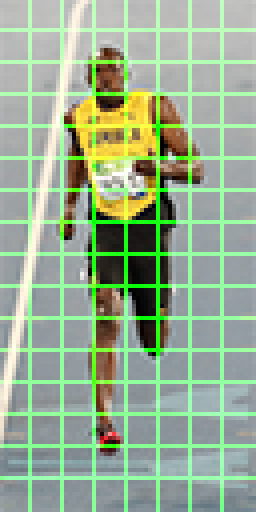
\includegraphics[width=0.2\textwidth]{./img/hog-cells}
	}
	\hfill
	\caption{The (a) descriptor blocks formed by the gradient histograms and (b) the devision of descriptor blocks. \cite{mallick_histogram_2016}}
	\label{fig:HOGBins}
\end{figure}

\subsection{Block Normalization}
\simpleparagraph{}
Once the gradient histograms have been produced, the magnitudes within each histogram needs to be normalized to its neighboring blocks. This allows for the features to be more invariant to dramatic pixel changes or irregularities. Instead of normalizing the entire $64\times 128$ size detection window, 4x4 blocks will be computed. These larger blocks concatenate the $9\times 1$ histogram vectors to a $36\times 1$ vector. The 4x4 norm block will traverse through the entire image by only moving one block horizontally or vertically at a time, see Figure \ref{fig:HOGBins}

\subsection{Finalize - Support Vector Machines}
\simpleparagraph{}
Once the blocks have been normalized, the $36\times 1$ vectors will be concatenated into one large $3780\times 1$ vector that is sent off to a Support Vector Machine. A Support Vector Machine or SVM is a machine learning technique that binaurally classifies objects. In other words, given some data set of only positive objects or training set and an input of new objects, a SVM will provide the set of new objects that are classified as matching the training set. In the case of HOG, the objects will be the HOG features of each image.

\section{Further Research}
\simpleparagraph{}
The topics and concepts covered in this paper are merely the tip of the iceberg, and it is highly recommended that further study be done in the fields of applied math. A number of textbooks were used in the writing of the paper, and would be helpful resources. The two most significant are \cite[Computer Vision: Algorithms and Application][]{szeliski_computer_2011} and \cite[Elementary Linear Algebra with Applications][]{kolman_elementary_2008}. Linear Algebra is the base for many of the concepts within computer vision and ought to be further reviewed. Szeliski's book on computer vision is one of the most well cited pieces of literature within the field of computer vision. It is a book that ought to be read after some of the \textit{mathematical groundwork} has been laid.

\nocite{*}
\newpage
\singlespacing
%\listoffigures
%\newpage
%Bibliography
\bibliographystyle{IEEEtranN}
\phantomsection
\addcontentsline{toc}{section}{Bibliography} 
\bibliography{Citations}

\end{document}